\documentclass[reprint,english]{revtex4-1}

% language
\usepackage[utf8]{inputenc}
\usepackage[english]{babel}

% standard setup
\usepackage{physics,amssymb,array}
\usepackage{xcolor,graphicx,hyperref}
\usepackage{tikz,listings,multirow}
\usepackage{subfigure}
\usepackage{enumitem}

% hyperref coloring
\hypersetup{ %
  colorlinks,
  linkcolor={red!50!black},
  citecolor={blue!50!black},
  urlcolor={blue!80!black}}

% lstlisting coloring
\lstset{ %
  inputpath=,
  backgroundcolor=\color{white!88!black},
  basicstyle={\ttfamily\scriptsize},
  commentstyle=\color{magenta},
  language=C++,
  tabsize=2,
  stringstyle=\color{green!55!black},
  frame=single,
  keywordstyle=\color{blue},
  showstringspaces=false,
  columns=fullflexible,
  keepspaces=true}

% pretty matrix
\newcolumntype{C}[1]{>{\centering\arraybackslash$}p{#1}<{$}}

% simplify
\newcommand{\Ham}{\hat{\mathcal{H}}}

\begin{document}
% titlepage
\title{FYS3150 Report\\Project 2 - Solving Eigenvalue Problems}
\author{Nils Johannes Mikkelsen}
\date{\today}
\noaffiliation
\begin{abstract}
something abstract
\end{abstract}
\maketitle

% body
\section*{About Project 2}
This is a report for Project 2 in FYS3150 Computational Physics at UiO, due October \(1^{\text{st}}\), 2018. \cite{project2} The project description was accessed September\(22^{\text{nd}}\), 2018 with the following web address:\\
{\scriptsize\url{https://github.com/CompPhysics/ComputationalPhysics/blob/master/doc/Projects/2018/Project2/pdf/Project2.pdf}}\\
All material written for this report can be found in this GitHub repository:\\
{\scriptsize\url{https://github.com/njmikkelsen/comphys2018/tree/master/Project2}}
\section{Introduction}
Project 2 in FYS3150 Computational Physics is concerned with the problem of solving eigenvalue problems, in particular matrix eigenvalue problems. However, instead of solving arbitrary eigenvalue problems, this report will investigate some important examples from physics: the buckling beam and the radial harmonic oscillator. Most of the equations are already on the eigenvalue-problem format. However, further treatment will bring the equations to dimensionsless form in order to highlight their underlying similarities, especially in the context of solving them by numerical means. In the following sections, all the continuous problems will be introduced before the discretisation process.

The matrix eigenvalue equations will be solved using the famous Jacobi eigenpair/diagonalisation algorithm, which is an essential algorithm in the field of numerical Linear Algebra. More modern methods (such as Householder's algorithm, etc.) have been proven to be much more effective than the Jacobi algorithm with respect accuracy, stability and computation-time. Nonetheless, the Jacobi algorithm is historically important and serves as a stepping stone for future study of more complex methods.

Having applied the algorithm to the simpler cases, the project will expand its horizon and study a Coulomb-interaction pair of electrons, situated in a harmonic oscillator potential.
\section{Theory}
All eigenvalue problems may be written as
\begin{equation}
\hat{\Lambda}f=\lambda f
\end{equation}
where \(f\) and \(\lambda\) is an eigenvector-eigenvalue eigenpair of the operator \(\hat{\Lambda}\). Other than requiring the existence of at least one eigenvector, the operator \(\hat{\Lambda}\) does not need to be restricted in any particular way.
\subsection{Eigenvalue Problems in Physics:\\The Buckling Beam}
A straight non-rigid beam of length \(L\) is fastened at \(x=0\) and \(x=L\). A constant uniform force \(\vb{F}=-F\vu{e}_x\) is applied to the beam at \(x=L\) such that the beam is bended in the \(\vu{e}_y\) direction with displacement \(y(x)\). Using infinitesimal analysis, one can show that the beam's bending behaves according to
\begin{equation}\label{eq:initial_buckling_beam}
\gamma\partial_x^2y(x)=-Fy(x)\qc x\in[0,L]
\end{equation}
where \(\gamma\) is a rigidity parameter and \(y(x)\) is restricted by Dirichlet boundary conditions \(y(0)=y(L)=0\).

The next step is to introduce the dimensionless variables \(\xi=x/L\) and \(v(\xi)=y(L\xi)\), which by definition implies that \(\xi\in[0,1]\). The new Dirichlet boundaries become \(v(0)=v(1)=0\) and the eigenvalue equation may be written as
\begin{equation}\label{eq:dimless_buckling_beam}
\partial_{\xi}^2v(\xi)=-\lambda v(\xi)
\end{equation}
Here, \(v(\xi)\) are eigenvectors with corresponding eigenvalues \(-\lambda=FL^2/\gamma\).
\subsection{Eigenvalue Problems in Physics:\\The Radial Schrödinger Equation}\label{sec:radial_scrodinger_equation}
Provided the spherical coordinates basis \(\{\ket{r,\theta,\varphi}\}\), the Hamiltonian for a particle of mass \(m\) in a spherically symmetric potential \(V(r)\) may be written as
\begin{equation}\label{eq:std_hamiltonian}
\Ham=\frac{-\hbar^2}{2m}\laplacian+V(\hat{r})
\end{equation}
where the laplacian is given by
\begin{equation}\label{eq:laplacian_spherical_coordinates}
\laplacian=r^{-1}\partial_r^2r+r^{-2}\Big(\csc\theta\partial_\theta[\sin\theta\partial_\theta]+\csc^2\theta\partial_\varphi^2\Big)
\end{equation}
Using the canonical operatores \(\hat{x}=x\) and \(\hat{p}=-i\hbar\nabla\), one can show that the angular momentum operator \(\vu{L}^2=\vu{L}_x^2+\vu{L}_y^2+\vu{L}_z^2\) is given by
\[\vu{L}^2=-\hbar^2\Big(\csc\theta\partial_\theta[\sin\theta\partial_\theta]+\csc^2\theta\partial_\varphi^2\Big)\]
which implies that the hamiltonian may be rewritten in terms of \(\vu{L}^2\):
\begin{equation}\label{eq:hamiltonian_via_L2}
\Ham=\frac{-\hbar^2}{2mr}\partial_r^2r+\frac{\vu{L}^2}{2mr^2}+V(\hat{r})
\end{equation}
All components of \(\Ham\) commutes, thus \([\Ham,\vu{L}^2]=0\). Therefore, \(\Ham\) and \(\vu{L}^2\) must share eigenstates \(\psi(r,\theta,\varphi)\). However, the eigenstates of \(\vu{L}^2\) are already known to be the spherical harmonics \(Y_\ell^m(\theta,\varphi)\), meaning that the \(r\)-dependency of \(\psi\) must be independent of \((\theta,\varphi)\). Or in other words:
\begin{equation}\label{eq:eigenstates_hamiltonian_L2}
\psi(r,\theta,\varphi)=\mathcal{R}(r)Y_\ell^m(\theta,\varphi)
\end{equation}

The eigenvalues of \(\vu{L}^2\) are \(\vu{L}^2Y_\ell^m(\theta,\varphi)=\hbar^2\ell(\ell+1)Y_\ell^m\). Thus, the eigenvalues of \(\Ham\) are determined by
\begin{align}
\Ham\psi&=E\psi\nonumber\\
\frac{-\hbar^2}{2mr}\partial_r^2r\psi+\frac{\hbar^2\ell(\ell+1)}{2mr^2}\psi+V(r)\psi&=E\psi\nonumber\\
\frac{-\hbar^2}{2mr}\partial_r^2r\mathcal{R}(r)+\frac{\hbar^2\ell(\ell+1)}{2mr^2}\mathcal{R}(r)+V(r)\mathcal{R}(r)&=E\mathcal{R}(r)\nonumber
\end{align}
i.e. the so-called Radial Schrödinger equation. The equation may be further simplified by introducing the transformation \(u(r)=r\mathcal{R}(r)\):
\begin{equation}\label{eq:radial_schrodinger_equation_simplified}
\frac{-\hbar^2}{2m}\partial_r^2u(r)+\Big[V(r)+\frac{\hbar^2\ell(\ell+1)}{2mr^2}\Big]u(r)=Eu(r)
\end{equation}
The Dirichlet boundary conditions for this equation are \(u(0)=\displaystyle\lim_{b\to\infty}u(b)=0\).

Finally, one may introduce the dimensionless variables \(\xi=r/\alpha\) and \(v(\xi)=u(\alpha\xi)\), where \(\alpha\) is the system's so-called natural length scale. Note that \(\xi\in[0,\infty)\) and that the Dirichlet boundary conditions for \(v(\xi)\) are completely equivalent to those of \(u(r)\). Equation \eqref{eq:radial_schrodinger_equation_simplified} may thus, via a little algebra, be rewritten as the dimensionless eigenvalue equation:
\begin{equation}\label{eq:dimless_radial_schrodinger}
\Big[\partial_\xi^2-\frac{2m\alpha^2}{\hbar^2}V(\alpha\xi)-\frac{\ell(\ell+1)}{\xi^2}\Big]v(\xi)=-\lambda v(\xi)
\end{equation}
Here, \(v(\xi)\) are eigenvectors with corresponding eigenvalues \(-\lambda=2m\alpha^2E/\hbar^2\).

It is now impossible to continue the analysis without specifying the potential energy function \(V(r)\).
\subsubsection{The harmonic oscillator potential}
The harmonic oscillator potential is given by \(V(r)=\frac{1}{2}m\omega^2r^2\). This implies that
\[\frac{2m\alpha^2}{\hbar^2}V(\alpha\xi)=\frac{m^2\omega^2}{\hbar^2}\alpha^4\xi^2\]
Now if \(\alpha=i\sqrt{\hbar/m\omega}\), then equation \eqref{eq:dimless_radial_schrodinger} simplifies to
\begin{equation}\label{eq:dimless_radial_schrodinger_harmonic_oscillator}
\Big[\partial_\xi^2-\xi^2-\ell(\ell+1)\xi^{-2}\Big]v(\xi)=-\lambda v(\xi)
\end{equation}
where \(-\lambda=2E/\hbar\omega\).

While it is possible to solve equation \eqref{eq:dimless_radial_schrodinger_harmonic_oscillator} analytically, this will not be done here. However, the resulting energy eigenvalues are given by:
\begin{equation}\label{eq:harmonic_oscillator_energies}
E_{nl}=\hbar\omega\bigg(2n+\ell+\frac{3}{2}\bigg)
\end{equation}
where \(n=0,1,\ldots\) and \(\ell=0,1,\ldots,n-1\). This implies that the analytic values for \(\lambda\) are
\begin{equation}\label{eq:harmonic_oscillator_dimless_eigenvalues}
\lambda_{nl}=4n+2l+3
\end{equation}
\subsubsection{Two Coulomb-interacting electrons in a harmonic oscillator potential}
To extend the case of a single particle to the case of two interacting particles, the Hamiltonian must change accordingly:
\begin{equation}\label{eq:hamiltonian_two_particles}
\Ham=\frac{\abs{\vu{p}_1}^2}{2m_1}+\frac{\abs{\vu{p}_2}^2}{2m_2}+V(\vu{r}_1,\vu{r}_2)
\end{equation}
where in the case of two electrons: \(m_1=m_2=m\). If placed in a harmonic oscillator potential, and allowed to interact via a Coulomb interaction, the potential for the electron-electron system is given by
\begin{equation}
V(\vu{r}_1,\vu{r}_2)=V_H(\vu{r}_1)+V_H(\vu{r}_2)+V_C(\vu{r}_1-\vu{r}_2)
\end{equation}
where
\[V_H(\vb{r})=\frac{1}{2}m\omega^2\abs{\vb{r}}^2\qand V_C=\frac{k}{\abs{\vb{r}}}\]
with \(k=e^2/4\pi\varepsilon_0\). In order to simplify the calculations, the following coordinate transformation is introduced:
\begin{equation}
\vb{R}=\frac{1}{2}\big(\vb{r}_1+\vb{r}_2\big)\qand\vb{r}=\vb{r}_1-\vb{r}_2
\end{equation}
Here, \(\vb{R}\) represents the center of mass while \(\vb{r}\) represents the electrons' relative frame of reference. Following standard definitions, the momenta \(\vb{P}\) and \(\vb{p}\) corresponding to \(\vb{R}\) and \(\vb{r}\) are defined as follows:
\begin{equation}
\vb{P}=\vb{p}_1+\vb{p}_2\qand\vb{p}=\vb{p}_1-\vb{p}_2
\end{equation}
Hence, by definition:
\begin{align*}
4\big|\vb{R}\big|^2+\abs{\vb{r}}^2&=2\Big(\abs{\vb{r}_1}^2+\abs{\vb{r}_2}^2\Big)\\
\big|\vb{P}\big|^2+\abs{\vb{p}}^2&=2\Big(\abs{\vb{p}_1}^2+\abs{\vb{p}_2}^2\Big)
\end{align*}
Using \(\vb{R}\), \(\vb{r}\), \(\vb{P}\) and \(\vb{p}\), one may rewrite the Hamiltonian:
\begin{equation}\label{eq:hamiltonian_two_particles_new}
\Ham=\frac{\big|\vu{P}\big|^2}{4m}+\frac{\abs{\vu{p}}^2}{4m}+m\omega^2\big|\vu{R}\big|^2+\frac{1}{4}m\omega^2|\vu{r}|^2+\frac{k}{|\vu{r}|}
\end{equation}
This may be further seperated into two components \(\Ham_R\) and \(\Ham_r\), which are dependent on \(\vu{R}\) and \(\vu{r}\) respectively. All components of \(\Ham\) commute, thus \(\Ham_R\) and \(\Ham_r\) must share eigenstates \(\psi\). Provided the spherical coordinate bases \(\{\ket{R,\theta_R,\varphi_R}\}\) and \(\{\ket{r,\theta_r,\varphi_r}\}\), the eigenstates may be written in terms of two separate components:
\begin{equation}
\psi(\vb{R},\vb{r})=\phi(\vb{R})\chi(\vb{r})
\end{equation}
Moreover, the eigenvalue equation \(\Ham\psi=E\psi\) may be simplified via the separation of variables technique (the details have been omitted):
\begin{subequations}
\begin{align}
E_R+E_r&=E\\
\bigg[\frac{-\hbar^2}{4m}\laplacian_R+m\omega^2R^2\bigg]\phi=\Ham_R\phi&=E_R\phi\label{eq:separated_variables_eq1}\\
\bigg[\frac{-\hbar^2}{4m}\laplacian_r+\frac{1}{4}m\omega^2r^2+\frac{k}{r}\bigg]\chi=\Ham_r\chi&=E_r\chi\label{eq:separated_variables_eq2}
\end{align}
\end{subequations}
By following the exact same approach as the one laid out earlier in this section, the operators \(\laplacian_R\) and \(\laplacian_r\) may be rewritten in terms of \(\vu{L}_R^2\) and \(\vu{L}_r^2\) respectively. It follows that \(\Ham_R\) and \(\Ham_r\) commute with \(\vu{L}_R^2\) and \(\vu{L}_r^2\) such that \(\phi\) and \(\chi\) may be written as products of a radial component and spherical harmonics respectively:
\begin{subequations}
\begin{align}
\phi(R,\theta_R,\varphi_R)&=\mathcal{R}_R(R)Y(\ell_R,m_R;\theta_R,\varphi_R)\\
\chi(r,\theta_r,\varphi_r)&=\mathcal{R}_r(r)Y(\ell_r,m_r;\theta_r,\varphi_r)
\end{align}
\end{subequations}
As a result, equations \eqref{eq:separated_variables_eq1} and \eqref{eq:separated_variables_eq2} yield:
\begin{align*}
\bigg(\frac{-\hbar^2}{4mR}\partial_R^2R+m\omega^2R^2+\frac{\hbar^2\ell_R(\ell_R+1)}{4mR^2}\bigg)\mathcal{R}_R&=E_R\mathcal{R}_R\\
\bigg(\frac{-\hbar^2}{4mr}\partial_r^2r+\frac{1}{4}m\omega^2r^2+\frac{\hbar^2\ell_r(\ell_r+1)}{4mr^2}+\frac{k}{r}\bigg)\mathcal{R}_r&=E_r\mathcal{R}_r
\end{align*}
Again, introduce transformations \(u_R(R)=R\mathcal{R}_R(R)\) and \(u_r(r)=r\mathcal{R}_r(r)\) such that
\begin{align*}
\bigg(\frac{-\hbar^2}{4m}\partial_R^2+m\omega^2R^2+\frac{\hbar^2\ell_R(\ell_R+1)}{4mR^2}\bigg)u_R&=E_Ru_R\\
\bigg(\frac{-\hbar^2}{4m}\partial_r^2+\frac{1}{4}m\omega^2r^2+\frac{\hbar^2\ell_r(\ell_r+1)}{4mr^2}+\frac{k}{r}\bigg)u_r&=E_ru_r
\end{align*}
The \(R\)-equation is actually the same as the harmonic oscillator studied above. To realise this, one must introduce the dimensionless variables \(\xi=R/\alpha\) and \(v_R(\xi)=u_R(\alpha\xi)\), now with \(\alpha=i\sqrt{\hbar/2m\omega}\). In doing so the \(R\)-equation reduces to equation \eqref{eq:dimless_radial_schrodinger_harmonic_oscillator} with \(E_R=E\) and \(\lambda_R=2E/\hbar\omega\). This implies \(E_R\) is given by equation \eqref{eq:harmonic_oscillator_energies} and \(\lambda_R\) is given by equation \eqref{eq:harmonic_oscillator_dimless_eigenvalues}.

To continue with the \(r\)-equation, dimensionless variables \(\rho=r/\beta\) and \(v_r(\rho)=u_r(\beta\rho)\) are introduced:
\begin{align*}
\bigg(\partial_\rho^2-\frac{m^2\omega^2}{\hbar^2}\beta^4\rho^2-\frac{\ell_r(\ell_r+1)}{\rho^2}-\frac{4mk\beta}{\hbar^2\rho}\bigg)v_r\\=-\frac{4m\beta^2}{\hbar^2}E_rv_r
\end{align*}
At this point, \(\beta\) may be chosen in order to scale the equation either according to the harmonic oscillator potential or the Coulomb interaction. In an experimental setting, a harmonic oscillator potential could be adjustable whereas the Coulomb interaction is fixed. This implies that the Coulomb interaction serves best as the system's natural scale: \(\beta=\hbar^2/4mk\). Now let \(\omega_r^2=m^2\omega^2\beta^4/\hbar^2\) denote an adjustable dimensionless oscillatory parameter such that the final eigenvalue equation becomes
\begin{equation}\label{eq:dimless_two_particle_interaction}
\Big(\partial_\rho^2-\omega_r^2\rho^2-\ell_r(\ell_r+1)\rho^{-2}-\rho^{-1}\Big)v_r=-\lambda_rv_r
\end{equation}
Here, \(v_r(\rho)\) are eigenvectors with corresponding eigenvalues \(-\lambda_r=\hbar^2E_r/4mk^2\).

In conclusion, the total energy of the electron-electron system is given by
\begin{equation}
E=E_R+E_r=\hbar\omega\bigg(2n_R+\ell_R+\frac{3}{2}\bigg)-\frac{4mk^2}{\hbar^2}\lambda_r
\end{equation}

\subsection{Eigenvalues Of Tridiagonal Matrices}
The following theorem will not be proven here, but is included due to its comparative applications in this project.

Provided the following tridiagonal matrix equation:
\begin{equation}
\hat{A}\hat{\vb{x}}=\lambda\hat{\vb{x}}
\end{equation}
where \(\lambda\in\mathbb{R}\), \(\hat{\vb{x}}^T=\mqty[x_1&\cdots&x_n]\) and \(\hat{A}\) is composed by a central, upper and lower diagonal diagonal. All elements along the central diagonal are equal to \(b\), while all elements along the upper and lower diagonals are equal to \(a\).
The eigenvalues are given by
\begin{equation}\label{eq:tridiag_matrix_equation_eigenvalues}
\lambda_i=b+2a\cos\bigg[\frac{i\pi}{n+1}\bigg]\qfor i=1,2,\ldots,n
\end{equation}
\subsection{Discretisation}\label{sec:discretisation}
Let \(\xi\in[a,b]\) denote an independent variable and \(v(\xi)\in\mathbb{R}\) denote a dependent variable that satisfies some eigenvalue equation \(\hat{\Lambda} v(\xi)=\lambda v(\xi)\), where the variables and the operator are continuous objects. The operator may be a linear combination of several operators \(\hat{\Lambda}=\hat{\Lambda}_1+\hat{\Lambda}_2+\cdots\). The following section is concerned with the discretisation of these variables and operators.
\subsubsection{The variables}
The first step is to discretise the \(\xi\)-interval \([a,b]\) into \(n+1\) slices such that \(\xi\) is replaced by a grid with \(n+2\) \(\xi_i\) values:
\begin{equation}
\xi_i=a+ih\qfor i=0,1,\ldots,n+1
\end{equation}
where
\begin{equation}
h=\frac{b-a}{n+1}
\end{equation}
(Note that \(\xi_0=a\) and \(\xi_{n+1}=b\).) Following the discretisation of \(\xi\), \(v(\xi)\) is now naturally discretised as follows:
\begin{equation}
v_i=v(\xi_i)\qfor i=0,1,\ldots,n+1
\end{equation}
Any Dirichlet boundary conditions \(v(a)=v_a\) and \(v(b)=v_b\) are then imposed by setting \(v_0=v_a\) and \(v_{n+1}=v_b\). As opposed to the continuous variable \(v(\xi)\), the simplest way to represent the discrete variable-set \(\{v_i\}_{i=0}^{i=n+1}\) is as a column vector:
\begin{equation}
\vb{v}=\mqty(v_0&v_1&\cdots&v_{n+1})^T
\end{equation}
\subsubsection{Operator: The second derivative}
As \(\vb{v}\) is not a continous object, it is incompatible with the continous second derivative operator \(\hat{\Lambda}=\partial_\xi^2\). To work around this problem, the derivative must be approximated via some discretisation process. One such approach is the finite difference approximation, in particular the central finite difference approximation method for second order derivatives:

Consider the Taylor expansion of any single-variable function \(f(y)\), centered about \(y=x\):
\begin{align}
f(y)&= f(x)+f'(x)(y-x)+\frac{f''(x)}{2}(y-x)^2\nonumber\\
&\quad +\frac{f'''(x)}{6}(y-x)^3+\frac{f^{(4)}(x)}{24}(y-x)^4+\cdots\label{eq:second_order_taylor_expansion}
\end{align}
Now consider \(f(x\pm h)\):
\begin{align}
f(x\pm h)&=f(x)\pm f'(x)h+\frac{f''(x)}{2}h^2\nonumber\\
&\quad \pm\frac{f'''(x)}{6}h^3+\frac{f^{(4)}(x)}{24}h^4+\cdots
\end{align}
It follows that
\begin{align*}
&f(x+h)+f(x-h)=2f(x)+f''(x)h^2+\order{h^4}
\end{align*}
where it assumed that \(h\leq1\). The central finite difference approximation for second order derivatives is now found by solving for \(f''(x)=\partial_y^2f(x)=\partial_x^2f(x)\):
\begin{equation}\label{eq:second_order_finite_difference_approximation}
\partial_x^2f(x)=\frac{f(x+h)-2f(x)+f(x-h)}{h^2}+\order{h^2}
\end{equation}
(Note that the \emph{approximation} does not include the order-of term.) It is worth noting that equation \eqref{eq:second_order_finite_difference_approximation} is exact in the limit \(h\to0\):
\begin{align*}
\lim_{h\to0}\frac{f(x+h)-2f(x)+f(x-h)}{h^2}+\order{h^2}&=\\[2mm]
\lim_{h\to0}\frac{\frac{f(x+h)-f(x)}{h}-\frac{f(x)-f(x-h)}{h}}{h}+\order{h^2}&=\\[2mm]
\lim_{h\to0}\frac{f'(x+h)-f'(x)}{h}+\order{h^2}&=f''(x)
\end{align*}
The idea of equation \eqref{eq:second_order_finite_difference_approximation} is to approximate \(v''(\xi_i)\) for each \(i=1,\ldots,n\):
\begin{align*}
v''(\xi_1)&\approx h^{-2}\big(v_0-2v_1+v_2\big)\\
v''(\xi_2)&\approx h^{-2}\big(v_1-2v_2+v_3\big)\\
&\qquad\vdots\qquad\vdots\qquad\\
v''(\xi_n)&\approx h^{-2}\big(v_{n-1}-2v_n+v_{n+1}\big)
\end{align*}
Note that \(v''(\xi_0)\) and \(v''(\xi_{n+1})\) cannot be approximated as \(v_{-1}\) and \(v_{n+2}\) are unknown. The above equations may be written as a matrix equation if the second derivatives are denoted as the column vector \(\vb{v}''=\mqty(v''(\xi_1)&\cdots&v''(\xi_n))^T\):
\begin{align*}
\mqty(v''(\xi_1)\\\vdots\\v''(\xi_n)) &= h^{-2}
\mqty(1      & -2      & 1       & 0      & \cdots &  0       & 0        & 0      \\
      0      &  1      & -2      & 1      & \cdots &  \vdots  & \vdots   & \vdots \\
      0      &  0      & 1       & \ddots & \ddots &  \vdots  & \vdots   & \vdots \\
      \vdots &  \vdots & \vdots  & \ddots & \ddots &  1       &  0       & 0      \\
      \vdots &  \vdots & \vdots  & \cdots & 1      & -2       &  1       & 0      \\
      0      &  0      & 0       & \cdots & 0      & 1        &  -2      & 1       )
\mqty(v_0\\v_1\\\vdots\\v_n\\v_{n+1})
\end{align*}
Or simply
\begin{equation}\label{eq:discretised_second_derivative}
\vb{v}''=\hat{\Lambda}_D\vb{v}
\end{equation}
where \(\hat{\Lambda}\) is the giant matrix, including the factor \(h^{-2}\). Note that while \(\vb{v}\) contains \(n+2\) points, \(\vb{v}''\) only contains \(n\) points; this is also evident from the fact that \(\hat{\Lambda}_D\) is an \(n\times(n+2)\) matrix. \footnote{The fact that \(\hat{\Lambda}_D\) is an \(n\times(n+2)\) matrix implies that it accepts an \((n+2)\)-dimensional column vector and returns an \(n\)-dimensional column vector.} Furthermore, equation \eqref{eq:discretised_second_derivative} is the discrete equivalent to the continous equation:
\[\partial_\xi^2v(\xi)=v''(\xi)\]
As the local truncation error in each finite difference approximation is of order \(h^2\), and there are \(n\) approximations, the global truncation error goes as \(n\order{h^2}\cong \order{h}\). Hence, \(\hat{\Lambda}_D\) makes a truncation error of order \(h\) when it is used to approximate the continuous second derivative operator.
\subsubsection{Operator: Multiplication with another function}
A "multiplication-with-another-function operator" may be written as \(\hat{\Lambda}=g(\xi)\). Compared to the second derivative operator, these operators are much more simple to account for as they do not act on the eigenvector itself. The discretisation of these operators is simply given by \(\hat{\Lambda}_g=\text{diag}\mqty(g(\xi_0)\cdots g(\xi_{n+1})))\), which yields:
\begin{equation}
\hat{\Lambda}_g\vb{v}=\mqty[g(\xi_0)v_0 & \cdots & g(\xi_{n+1})v_{n+1}]^T
\end{equation}

A common example of these kind of operators are polynomials: \(g(\xi)=\xi^2\), \(g(\xi)=\xi^{-2}\), etc.

\subsection{Solving Matrix Eigenvalue Equations Via The Jacobi Algorithm}
The following section presents the Jacobi eigenpair/diagonalisation algorithm for solving matrix eigenvalue equations on the form:
\begin{equation}\label{eq:general_matrix_eigenvalue_problem}
\hat{A}\vb{v}=\lambda\vb{v}
\end{equation}
where \(\hat{A}\) is a symmetric matrix. The algorithm is based on the properties of similarity (orthogonal) transformations, and will therefore be dealt with first.
\subsubsection{Similarity transformations}
A symmetric matrix \(\hat{A}\in\mathbb{R}^{n\times n}\) is said to be similar to another symmetric matrix \(\hat{B}\in\mathbb{R}^{n\times n}\) if there exist a unitary matrix \(\hat{S}\in\mathbb{R}^{n\times n}\) that is such that
\begin{equation}\label{eq:definition_similar_matrix}
\hat{B}=\hat{S}^T\hat{A}\hat{S}
\end{equation}
Let \(\{\vb{u}_i\}_{i=1}^{i=n}\) denote an orthonormal basis for the column space of \(\hat{A}\): \(\vb{u}_i^T\vb{u}_j=\delta_{ij}\). The similarity transformation \(\vb{w}_i=\hat{S}^T\vb{u}_i\) preserves the orthonormality of the basis:
\[\vb{w}_i^T\vb{w}_j=\big(\hat{S}^T\vb{u}_i\big)^T\big(\hat{S}^T\vb{u}_j\big)=\vb{u}_i^T\hat{S}\hat{S}^T\vb{u}_j=\vb{u}_i^T\vb{u}_j=\delta_{ij}\]

The idea is to perform \(m\) number of transformations such that \(\hat{A}\) is diagonalised to \(\hat{D}\):
\begin{equation}
\hat{D}=\hat{S}_m^T\hat{S}_{m-1}^T\cdots\hat{S}_1^T\hat{A}\hat{S}_1\cdots\hat{S}_{m-1}\hat{S}_m
\end{equation}
where
\begin{equation}
\hat{D}=\text{diag}\mqty(\lambda_1&\lambda_2&\cdots&\lambda_n)
\end{equation}
Matrices \(\hat{S}_1,\ldots,\hat{S}_m\) are guaranteeed to exist as \(\hat{A}\) is a real symmetric matrix (the proof is not included here). Using \eqref{eq:definition_similar_matrix}, equation \eqref{eq:general_matrix_eigenvalue_problem} yields:
\[\hat{S}^T\hat{A}\hat{I}\vb{v}=\hat{S}^T\lambda\vb{v}\implies\hat{S}^TA\hat{S}\hat{S}^T\vb{v}=\lambda\hat{S}^T\vb{v}\implies\]
\begin{equation}\label{eq:similarity_transformed_eigenvalue_problem}
\hat{B}\big(\hat{S}^T\vb{v}\big)=\lambda\big(\hat{S}^T\vb{v}\big)
\end{equation}
As \(\hat{A}\) is a real symmetric matrix, its eigenvectors \(\vb{v}_1,\ldots,\vb{v}_n\) form an orthogonal basis for its column space. And as the transformation \(\hat{S}^T\vb{v}\) conserves orthogonality, the final eigenvectors \(\hat{S}_1\cdots\hat{S}_m\vb{v}\) must also form an orthogonal basis for the column space of \(\hat{A}\). Furthermore, equation \eqref{eq:similarity_transformed_eigenvalue_problem} reveals that the eigenvalue \(\lambda\) of \(\hat{A}\) is unaffected by each transformation.

Now let
\begin{equation}
\hat{V}=\mqty[\vu{v}_1&\cdots&\vu{v}_n]=\hat{S}_1\cdots\hat{S}_m\hat{I}
\end{equation}
so that \(\hat{V}^T\hat{A}\hat{V}=\hat{D}\). This implies
\begin{subequations}
\begin{align}
\hat{A}\hat{V}&=\mqty[\hat{A}\vu{v}_1\cdots\hat{A}\vu{v}_n]\\
\hat{A}\hat{V}&=\hat{V}\hat{D}=\mqty[\lambda_1\vu{v}_1&\cdots&\lambda_n\vu{v}_n]
\end{align}
\end{subequations}
which proves that the eigenvectors of \(\hat{A}\) are the vectors \(\vu{v}_1,\ldots,\vu{v}_n\). As orthogonal transformations preserves normalisation, the set \(\{\vu{v}_i\}_{i=1}^{i=n}\) must also form an orthonormal basis for the column space of \(\hat{A}\).
\subsubsection{The algorithm}
The unitary matrix used in the Jacobi algorithm is the so-called Givens rotation matrix \(\hat{G}(k,l,\theta)\), which is a generalisation of the rotation-matrix for planar (2-dimensional) coordinate systems. The elements in \(\hat{G}(k,l,\theta)\) are given by
\begin{equation}\label{eq:Givens_rotation_matrix}
g_{ij}=\begin{cases}1,&i=j\notin\{k,l\} \\ \cos\theta,&i=j\in\{k,l\} \\ \sin\theta,&i=k,\,j=l \\ -\sin\theta,&i=l,\,j=k \\ 0,&otherwise\end{cases}
\end{equation}
Before continuing to the actual algorithm, consider first the transformation \(\hat{B}=\hat{G}^T\hat{A}\hat{G}\), where the elements of the symmetric matrices \(\hat{A}\) and \(\hat{B}\) are denoted by \(a_{ij}\) and \(b_{ij}\). The simplest case, i.e. with \(n=2\), is the following
\[\mqty(b_{11}&b_{12}\\b_{12}&b_{22})=\mqty(c&s\\-s&c)\mqty(a_{11}&a_{12}\\a_{12}&a_{22})\mqty(c&-s\\s&c)\]
That is:
\begin{align*}
b_{11}&=c^2\,a_{11}-2sc\,a_{12}+s^2\,a_{22}\\
b_{12}&=(c^2-s^2)a_{12}+sc(a_{22}-a_{11})\\
b_{22}&=s^2\,a_{11}+2sc\,a_{12}+c^2\,a_{22}
\end{align*}
So far, no criteria has been placed on the parameter \(\theta\). However, the Jacobi algorith designs the matrix \(\hat{G}\), and thereby \(\theta\), such that \(b_{12}=0\):
\[a_{11}-a_{22}=\frac{\cos^2\theta-\sin^2\theta}{\sin\theta\cos\theta}a_{12}=(\cot\theta-\tan\theta)a_{12}\]
Using the identity \(2\cot(2\theta)=\cot\theta-\tan\theta\) one finds:
\[\cot(2\theta)=\frac{a_{11}-a_{22}}{2a_{12}}\]
Let \(t=\tan\theta\) and \(\tau=\cot(2\theta)\) so that
\[2\tau=t^{-1}-t\implies t^2+2\tau\,t-1=0\]
Which further implies
\begin{equation}\label{eq:jacobi_algorithm_t}
t=-\tau\pm\sqrt{1+\tau^2}
\end{equation}
Having found \(t\), finding \(s\) and \(c\) is simple:
\begin{subequations}\label{eq:jacobi_algorithm_cs}
\begin{align}
c&=\frac{1}{\sec\theta}=\frac{1}{\sqrt{1+\tan^2\theta}}=\frac{1}{\sqrt{1+t^2}}\\
s&=\cos\theta\frac{\sin\theta}{\cos\theta}=ct
\end{align}
\end{subequations}
A special case of the transformation is when \(a_{12}=0\): it follows that \(\theta=\pi/4\) and thus \(c=1\), \(s=0\).

By increasing the dimensionality of the transformation from \(n=2\) to any arbitrary \(n\), only two extra cases arise: whether the element \(a_{ij}\) is affected or not depends on its location in the matrix.

The key detail is to realise how the structure of \(\hat{G}\) is related to the identiy matrix: other than the \(k^{\text{th}}\) and \(l^{\text{th}}\) columns and rows, \(\hat{G}\) is essentially an identity matrix. It follows that all elements \(a_{ij}\) where \(i,j\notin\{k,l\}\) seemingly interact with the identity matrix; leaving them unchanged after the transformation: \(b_{ij}=a_{ij}\).

Furthermore, the elements \(b_{kk}\), \(b_{ll}\) and \(b_{kl}\) are the same elements as in the \(n=2\) case. The generalised \(\tau\) is:
\begin{equation}\label{eq:jacobi_algorithm_tau}
\tau=\frac{a_{kk}-a_{ll}}{2a_{kl}}
\end{equation}
The remaining elements \(b_{ik}=b_{ki}\) and \(b_{il}=b_{li}\), where \(i\notin\{k,l\}\), can be derived from the observation that the matrix product \(\hat{G}^T\hat{A}\) only acts on the rows of \(\hat{A}\), while the matrix product \(\hat{A}\hat{G}\) only acts on the columns of \(\hat{A}\). By computing \(\hat{A}\hat{G}\) (details omitted here), one finds:
\[b_{ik}=ca_{ik}-sa_{il}\qand b_{il}=sa_{ik}+ca_{il}\]
In summary, the elements of \(\hat{B}\) are given by:
\begin{subequations}\label{eq:Givens_transformation_matrix}
\begin{alignat}{3}
b_{ij}&=a_{ij},&&i,j\notin\{k,l\}\\
b_{ik}&=ca_{ik}-sa_{il},&&i\notin\{k,l\}\\
b_{il}&=sa_{il}+ca_{il},&&i\notin\{k,l\}\\
b_{kk}&=c^2a_{kk}-2sca_{kl}+s^2a_{ll}&&\\
b_{ll}&=c^2a_{kk}+2sca_{kl}+s^2a_{ll}&&\\
b_{kl}&=0&&
\end{alignat}
\end{subequations}
After performing the transformation, the eigenvectors (i.e. \(\hat{V}=\mqty[\vu{v}_1&\cdots&\vu{v}_n]\)) must also be updated in order to remain eigenvectors for the transformed matrix:
\begin{equation}
\hat{V}_{new}=\hat{V}_{old}\hat{G}
\end{equation}
This operation exactly mirrors \(\hat{A}\hat{G}\), hence:
\begin{subequations}\label{eq:Givens_transformation_eigenvectors}
\begin{alignat}{2}
v_{ik}^{\text{new}}&=cv_{ik}^{\text{old}}-sv_{il}^{\text{old}},&\quad i\notin\{k,l\}\\
v_{il}^{\text{new}}&=sv_{il}^{\text{old}}+cv_{il}^{\text{old}},&\quad i\notin\{k,l\}
\end{alignat}
\end{subequations}

The Jacobi algorithm is essentially comprised of performing orthogonal transformations \(\hat{A}_{p+1}=\hat{G}^T\hat{A}_p\hat{G}\) until \(\hat{A}\) is "successfully diagonalised". As this process is iterative, true diagonalisation is only guaranteed in the limit \(p\to\infty\). In order to terminate the process, the quality of the diagonalisation must be measured by some criterion at the end of each iteration. A commonly used measure is whether the off-diagonal elements of \(\hat{A}_p\) are sufficiently small:
\begin{equation}\label{eq:off_diagonal_frobenius}
\text{off}(\hat{A})=\sqrt{\sum_{i=1}^n\sum_{j\neq i}^na_{ij}^2}\leq\epsilon
\end{equation}
for some error tolerance \(\epsilon\). However, it is computationally very ineffective to require the computation of \(\text{off}(\hat{A})\) at each iteration. Instead, consider the following:
\begin{equation}\label{eq:off_diagonal_with_max}
\text{off}(\hat{A})\leq\sqrt{\sum_{i=1}^n\sum_{j\neq i}^n\max\{a_{ij}^2\}}=n\max\{|a_{ij}|\}
\end{equation}
Finding \(n\max\{|a_{ij}|\}\) is much more computation-friendly and is thus better suited for the algorithm. As \(n\) simply scales the tolerance, the essential measure is:
\begin{equation}\label{eq:jacobi_algorithm_tolerance}
\max\{|a_{ij}|\}\leq\varepsilon
\end{equation}
The number of iterations required to satisfy \eqref{eq:jacobi_algorithm_tolerance} is difficult to quantify. In order to avoid unpredictably long computation time, a maximum number of iterations \(N_{\text{max}}\) is also enforced in the algorithm.

Due to the miniscule effects of the transformation (it only affects the \(k^{\text{th}}\) and \(l^{\text{th}}\) columns and rows), the choice of coefficients \(k\) and \(l\) becomes very important. Seeing that the transformation defines \(b_{kl}=0\), a clever approach would be to choose \(k\) and \(l\) using \(\max\{|a_{ij}|\}\). This approach is also the most effective with respect to equation \eqref{eq:jacobi_algorithm_tolerance} in that each step reduces the current \(\max\{|a_{ij}|\}\) to zero.

The full Jacobi-diagonalisation algorithm can be summaried as follows:
\begin{enumerate}
\item Set \(p=0\), load \(\hat{A}_0\) and define \(\hat{V}=\hat{I}\).
\item Compute \(a_{kl}=a_{max}=\max\{|a_{ij}|\}\).
\item \texttt{while} \(\max\{|a_{ij}|\}>\varepsilon\,\) \texttt{and} \(p\leq N_{\text{max}}\):
	\begin{itemize}
	\item[]Compute \(\tau\), \(t\), \(c\) and \(s\) using equations \eqref{eq:jacobi_algorithm_tau}, \eqref{eq:jacobi_algorithm_t} and 	\eqref{eq:jacobi_algorithm_cs} respectively.
	\item[]Use equations \eqref{eq:Givens_transformation_matrix} to adjust \(\hat{A}_{p+1}\).
	\item[]Use equations \eqref{eq:Givens_transformation_eigenvectors} to adjust \(\hat{V}_{p+1}\).
	\item[]Find \(a_{kl}=a_{max}=\max\{|a_{ij}|\}\).
	\item[]\(p=p+1\).
	\end{itemize}
\item Extract
\[\mqty[\lambda_1&\cdots&\lambda_n]=\text{diag}(\hat{A}_p)\qand\mqty[\vu{v}_1&\cdots&\vu{v}_n]=\hat{V}\]
\end{enumerate}

\section{Method}
\subsection{Testing The Machinery On The Buckling Beam}
This first problem serves mainly as a test for both the Jacobi algorithm and the mathematical formalism developed in the theory section. The existence of simple analytic eigenvalues makes the problem an excellent starting point.

Equation \eqref{eq:dimless_buckling_beam}, which governs the system, contains the second derivative operator \(\partial_\xi^2\). Employing the discretisation formalism yields the equation
\begin{equation}\label{eq:discrete_dimless_buckling_beam}
\hat{\Lambda}_D\vb{v}=-\lambda\vb{v}
\end{equation}
However, by imposing the Dirichlet boundary conditions \(v_0=v_{n+1}=0\) it is apparent that the first and last columns of \(\hat{\Lambda}_D\) serves no purpose. Ignoring these columns results in the symmetric tridiagonal matrix eigenvalue equation:
\begin{equation}\label{eq:method:buckling_beam}
D\tilde{\vb{v}}=-\lambda\tilde{\vb{v}}
\end{equation}
where \(D\) is the symmetric tridiagonal matrix (without the \(h^2\) term), \(\tilde{\vb{v}}=h^2\mqty(v_1&\cdots&v_n)^T\) and the analytic eigenvalues \(-\lambda\) are given by equation \eqref{eq:tridiag_matrix_equation_eigenvalues}.

Equation \eqref{eq:method:buckling_beam} is solved using the Jacobi algorithm for all combinations of \(\varepsilon\in\{10^{-2},10^{-6},10^{-10}\}\) and \(n\in\{10,100,300\}\), where \(N_\text{max}\) is increased beyond the necessary amount of iterations. Our interest lies in the accuracy of the Jacobi algorithm. The simplest criteria to tell whether the algorithm is successful is to compare the eigenvalues to the analytic eigenvalues.

In order to add an additional layer of confidence to the accuracy of the algorithm, the same system will be analysed using the \texttt{eig\_sym} function from the \texttt{Armadillo C++} library.
\subsection{Evaluating The Discrete Formalism Via The Quantum Harmonic Oscillator Potential}
Having succesfully completed a preliminary test of the algorithm, the machinery is now put to work on the quantum harmonic oscillator system, i.e. equation \eqref{eq:dimless_radial_schrodinger_harmonic_oscillator}. Whereas the buckling beam system featured definite variable boundaries \(0\leq\xi\leq1\), the harmoni oscillator system does not: \(0\leq\xi<\infty\). Seeing that this is impossible to represent using a grid, infinity must be approximated by some upper boundary \(\xi_\infty\). The goal is to study how the discrete mathematics behaves with respect to the parameters \(\xi_\infty\) and \(n\). 

To simplify the interpretations, the azimuthal quantum number is set to zero: \(\ell=0\). The remaining operators in \eqref{eq:dimless_radial_schrodinger_harmonic_oscillator} are thus the second derivative operator \(\partial_\xi^2\) and a multiplication-operator \(-\xi^2\). Employing the discretisation formalism yields:
\begin{equation}\label{eq:discrete_dimless_harmonic_oscillator}
\Big[\hat{\Lambda}_D+\hat{\Lambda}_g\Big]\vb{v}=-\lambda\vb{v}
\end{equation}
where \(g(\xi)=-\xi^2\). By imposing the boundary conditions \(v(0)=v(\xi_\text{upper})=0\), the first and final columns of \(\hat{\Lambda}_D\) is again found to be unecessary. The resulting tridiagonal matix may therefore be combined with \(\hat{\Lambda}_g\) (which is diagonal) to produce the tridiagonal matrix equation:
\begin{equation}\label{eq:method:quantum_harmonic_oscillator}
E\tilde{\vb{v}}=-\lambda\tilde{\vb{v}}
\end{equation}
where \(\tilde{\vb{v}}=h^2\mqty[v_1&\cdots&v_n]\) and \(E\) is a tridiagonal matrix whose coefficents are \(-2-h^2\xi_i^2\) along the central diagonal and 1 along both the upper and lower diagonals.

The problem will be studied for all combinations of \(\xi_\infty\in\{0.5,1,1.5,2,4\}\) and \(n\in\{10,100,500\}\), where \(\varepsilon=10^{-8}\) and \(N_\text{max}\) is increased beyond the necessary amount of iterations. 
\subsection{Applying The Machinery To The Electron-Electron System}
As a final challenge, the machinery will now be put to use on the Coulomb-interacting electrons that are located in a harmonic oscillator potential. Seeing that the center-of-mass frame is essentially just the one-dimensional harmonic oscillator, the focus in this report will lie on the relative frame (i.e. equation \eqref{eq:dimless_two_particle_interaction}).

Again the simplification \(\ell=0\) is assumed, meaning the remaining operators are: \(\partial_\rho^2\), \(-\omega^2\rho^2\) and \(-\rho^{-1}\), where \(\omega\) is a parameter. Once more infinity is approximated by some large value \(\rho_\infty\) such that the mathematical formalism yields:
\begin{equation}\label{eq:discrete_dimless_interacting_electrons}
\Big[\hat{\Lambda}_D+\hat{\Lambda}_{\tilde{g}}+\hat{\Lambda}_f\Big]\vb{v}=-\lambda\vb{v}
\end{equation}
where \(\tilde{g}(\rho)=-\omega_r^2\rho^2\) and \(f(\xi)=-\rho^{-1}\). Again \(\hat{\Lambda}_D\) may be simplified by imposing the boundary conditions \(v(0)=v(\rho_\text{upper})=0\), leading to the tridiagonal matrix
\begin{equation}\label{eq:method:interacting_electrons}
G\tilde{\vb{v}}=-\lambda\tilde{\vb{v}}
\end{equation}
where \(\tilde{\vb{v}}=h^2\mqty[v_1&\cdots&v_n]\) and \(G\) is a tridiagonal matrix whose coefficients are \(-2-h^2(\omega^2\rho^2+\rho^{-1})\) along the central diagonal and 1 along both the upper and lower diagonals.

The end-goal is study the balance between the Coulomb-interaction and the harmonic oscillator potential: while the Coulomb potential repels the electrons, the harmonic oscillator potential centers the electrons about the origin, thereby forcing them closer together. This balance will be studied via the parameter \(\omega\in\{\}\). Other parameters used in the program include \(n=300\), \(\varepsilon=10^{-8}\), sufficient \(N_\text{max}\) and a sufficient \(\rho_\infty\). \footnote{The use of ``sufficient'' here implies that the parameter is determined such that it has no affect on the results.} In order to gain some insight from the results, the resulting probability distributions \(p(\rho)=|v(\rho)|^2\) will be compared. However, to avoid unecessary confusion with the energy, only the ground state will be analysed.
\section{Results}
For the sake of not included 10 identical figures, only a handful of the prepared figures are featured. All figures, along with all other material, are available on at the github address:\\
{\scriptsize\url{https://github.com/njmikkelsen/comphys2018/tree/master/Project2}}
\subsection{The Buckling Beam}
A clear trend revealed itself whilst studying this system: the Jacobi algorithm is slow, however accurate. Moreover, it's accuracy is dependent on a sufficient user-defined tolerance \(\varepsilon\). Figure \ref{fig:bucklingbeam_eigenvectors1} shows an example with \(n=100\) and an error tolerence of only \(\varepsilon=10^{-2}\): the resulting eigenvector becomes terribly off. As long as the user is aware of this potential pitfall, this is not necessarily a big problem. Figure \ref{fig:bucklingbeam_eigenvectors2} shows another example with \(n=100\), however now with \(\varepsilon=10^{-10}\): the eigenvector comes out as expected.
\begin{figure}[h]
\centering
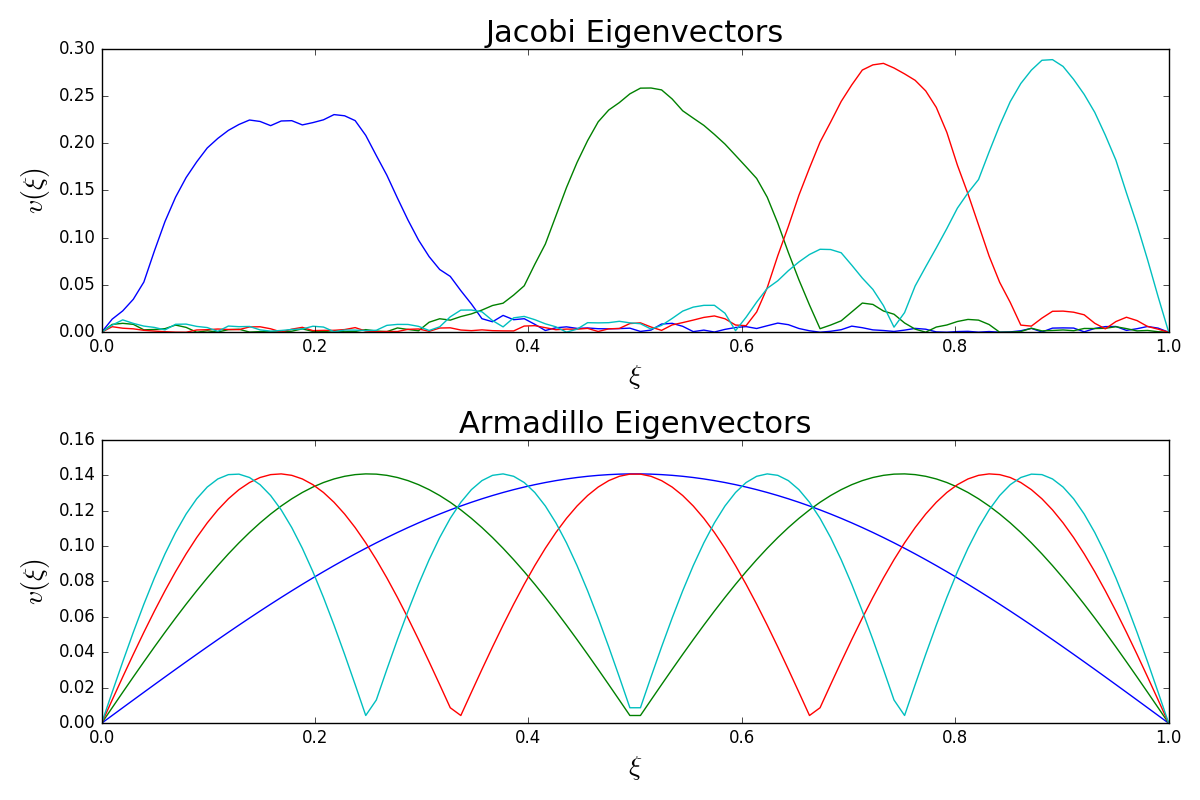
\includegraphics[scale=0.275]{BucklingBeam/plots/vector100_2.png}
\caption{Some eigenvectors of the Buckling Beam system. The numerical calculation defined \(n=100\) and \(\varepsilon=10^{-2}\).}
\label{fig:bucklingbeam_eigenvectors1}
\end{figure}
\begin{figure}[h]
\centering
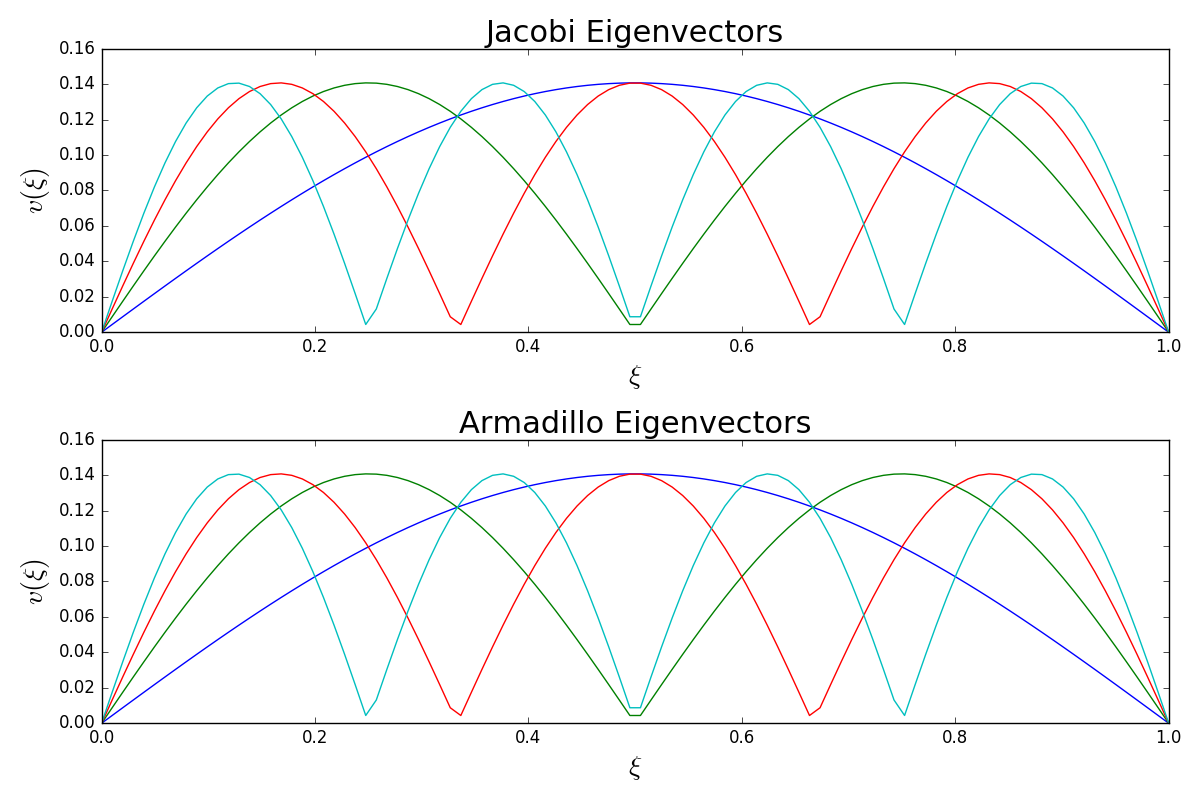
\includegraphics[scale=0.275]{BucklingBeam/plots/vector100_10.png}
\caption{Some eigenvectors of the Buckling Beam system. The numerical calculation defined \(n=100\) and \(\varepsilon=10^{-2}\).}
\label{fig:bucklingbeam_eigenvectors2}
\end{figure}

While some of the eigenvectors in computations with large \(\varepsilon\) turned out completely wrong, the eigenvalues matched the analytic eigenvalues very well in almost every computation. Table \ref{tab:bucklingbeam_MSE} shows a Mean Square Error (MSE) score for every computation: most notably there are no immediately critical errors. \texttt{armadillo} performs especially impressive with zero error within the specified precision, Jacobi performs also quite well.
\begin{table}[h]
\centering
\caption{Mean Square Error score for both the Jacobi-calculated eigenvalues and the \texttt{armadillo}-calculated eigenvalues for every computation of the Buckling Beam system. The figures have been truncated due to uneccesary precision.}\label{tab:bucklingbeam_MSE}
\begin{tabular}{|c|c|c|c|}
\hline
\(n\) & \(\varepsilon\) & Jacobi MSE             & \texttt{armadillo} MSE \\\hline
10    & \(10^{-2}\)     & \(1.34\cdot10^{-7}\)   & 0                      \\\hline
10    & \(10^{-6}\)     &  0                     & 0                      \\\hline
10    & \(10^{-10}\)    &  0                     & 0                      \\\hline
100   & \(10^{-2}\)     &  \(9.17\cdot10^{-4}\)  & 0                      \\\hline
100   & \(10^{-6}\)     &  \(1.00\cdot10^{-20}\) & 0                      \\\hline
100   & \(10^{-10}\)    &  0                     & 0                      \\\hline
300   & \(10^{-2}\)     &  \(6.82\cdot10^{-3}\)  & 0                      \\\hline
300   & \(10^{-6}\)     &  \(1.02\cdot10^{-16}\) & 0                      \\\hline
300   & \(10^{-10}\)    &  0                     & 0                      \\\hline
\end{tabular}
\end{table}
\subsection{The Harmonic Oscillator}
The importance of choosing an appropriate approximation of infinity can be summaried by figures \ref{fig:harmonicoscillator_eigenvectors1} and \ref{fig:harmonicoscillator_eigenvectors2}: While the major shape is conserved, the curvature of the wave functions are very distorted in figure \ref{fig:harmonicoscillator_eigenvectors1}. Figure \ref{fig:harmonicoscillator_eigenvectors2} on the other hand is much more generous with its infinity and yields therefore much more accurate results. One detail that is particulary noticeable between the two is the maximum height of the wave functions. Whereas all wave functions are more or less equally tall in figure \ref{fig:harmonicoscillator_eigenvectors1}, there is a clear difference between the different concentrations in figure \ref{fig:harmonicoscillator_eigenvectors2}.
\begin{figure}[h]
\centering
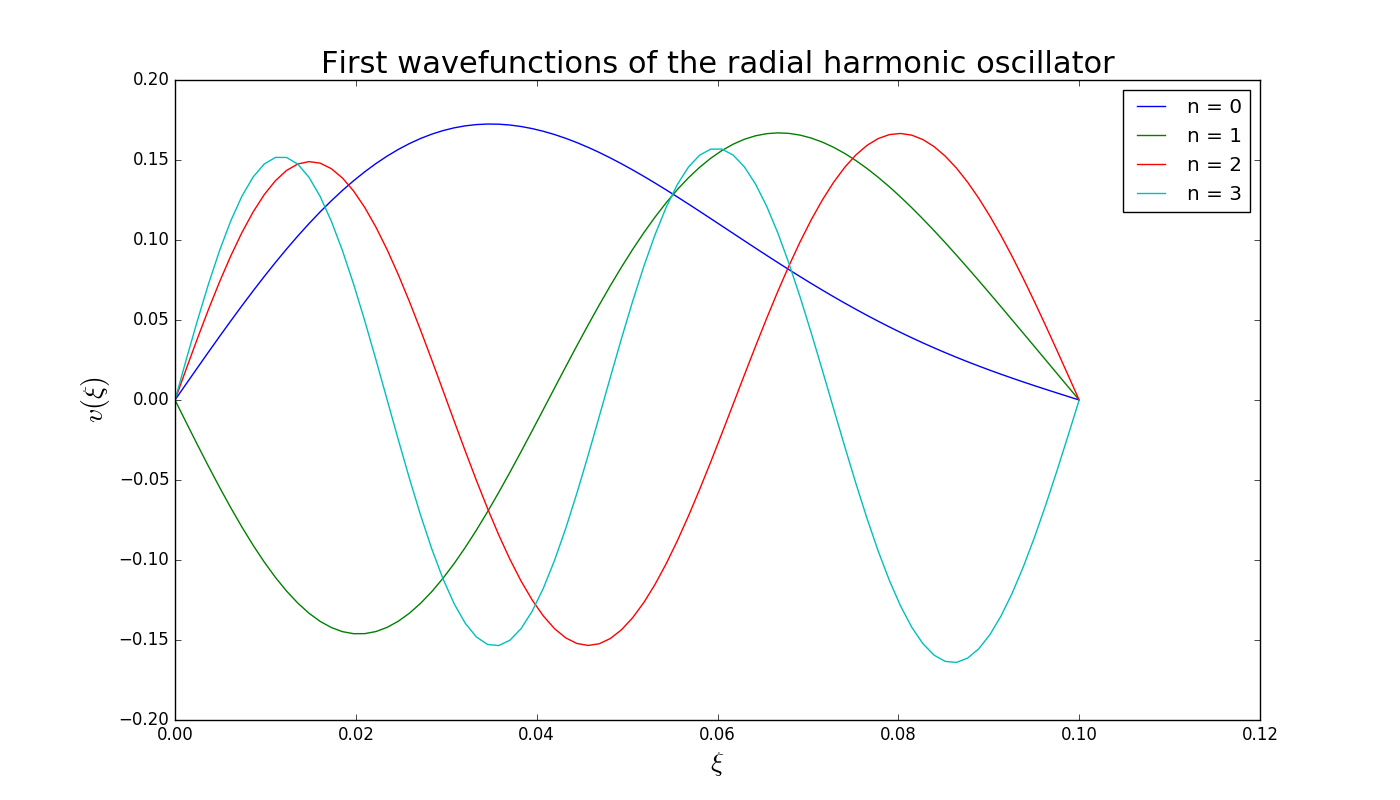
\includegraphics[scale=0.27]{HarmonicOscillator/plots/wavefunction80_1.png}
\caption{The first wavefunctions of the radial quantum harmonic oscillator. Here, infinity is approximated by \(\xi_\infty=0.1\).}
\label{fig:harmonicoscillator_eigenvectors1}
\end{figure}
\begin{figure}[h]
\centering
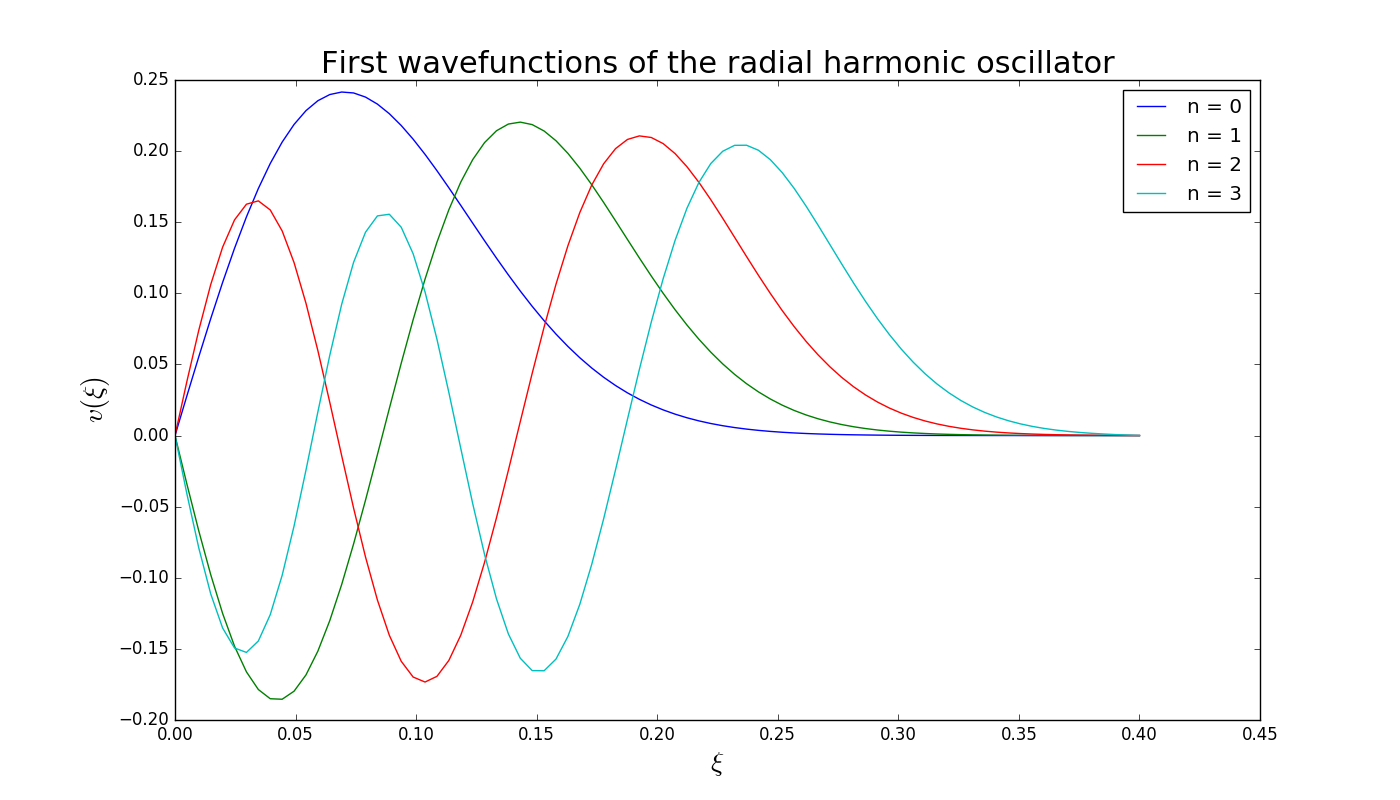
\includegraphics[scale=0.27]{HarmonicOscillator/plots/wavefunction80_4.png}
\caption{The first wavefunctions of the radial quantum harmonic oscillator. Here, infinity is approximated by \(\xi_\infty=0.4\).}
\label{fig:harmonicoscillator_eigenvectors2}
\end{figure}
\subsection{The Coulomb-Interacting Electron-Electron Harmonic Oscillator}
The effect of adjusting the harmonic oscillator frequency is immediately obvious from figures \ref{fig:interactingelectrons_eigenvectors1}, \ref{fig:interactingelectrons_eigenvectors2} and \ref{fig:interactingelectrons_eigenvectors3}: Increasing the frequency, which leads to a relative decrease in the repulsive Coulomb interaction, yields a concentration of the electrons. This is not surprising as there are only potentials working against each other: the Coulomb-interaction trying to pull the electrons a part, and the harmonic oscillator trying to concentrate the electrons about a common center. The relative increase in the strength of the harmonic oscillator is therefore expected to lead to a greater probability concentration closer to the origin.
\begin{figure}[h]
\centering
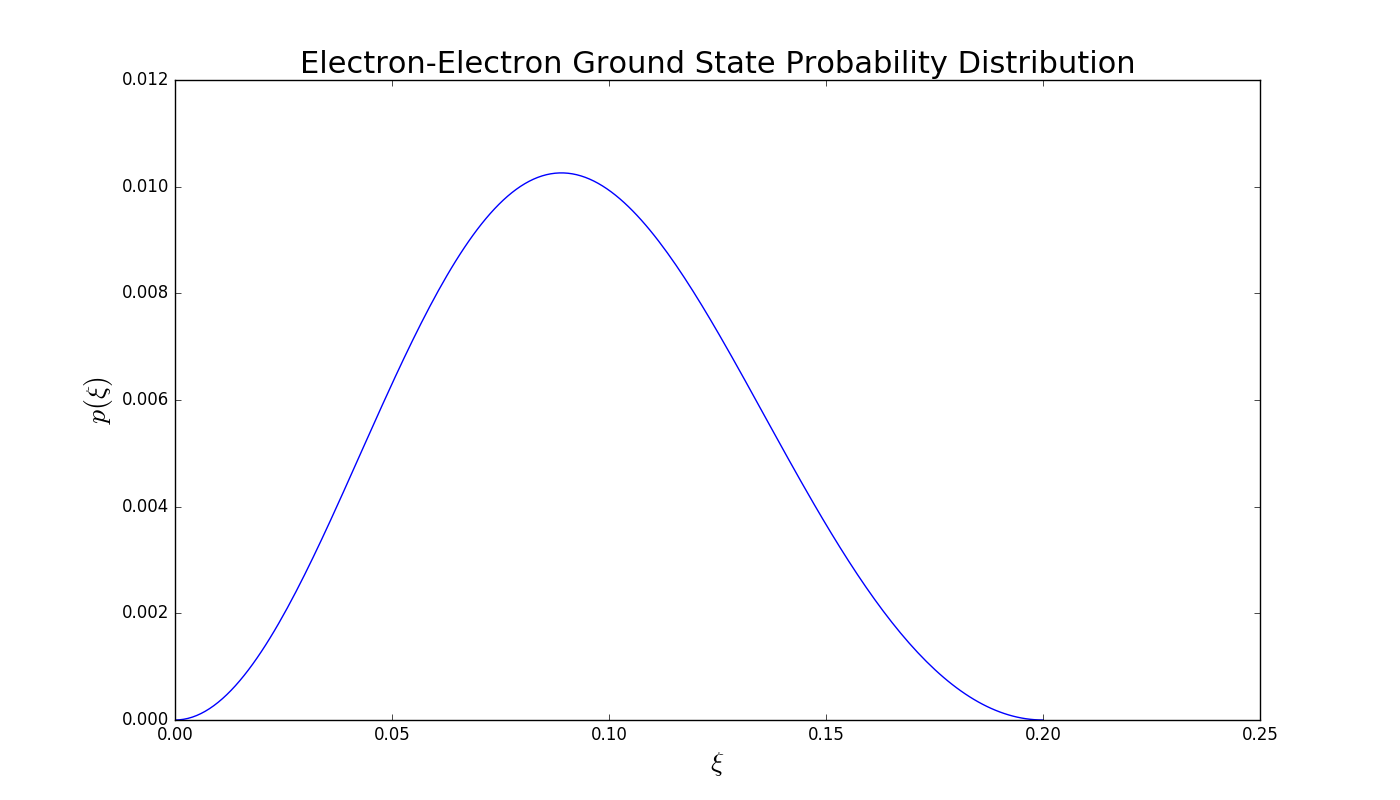
\includegraphics[scale=0.275]{InteractingElectrons/plots/prob200_1.png}
\caption{The radial ground state of the Coulomb-interacting electron-electron quantum harmonic oscillator. Here, infinity is approximated by \(\xi_\infty=0.2\) and the harmonic oscillator frequency is \(\omega=0.1\).}
\label{fig:interactingelectrons_eigenvectors1}
\end{figure}
\begin{figure}[h!]
\centering
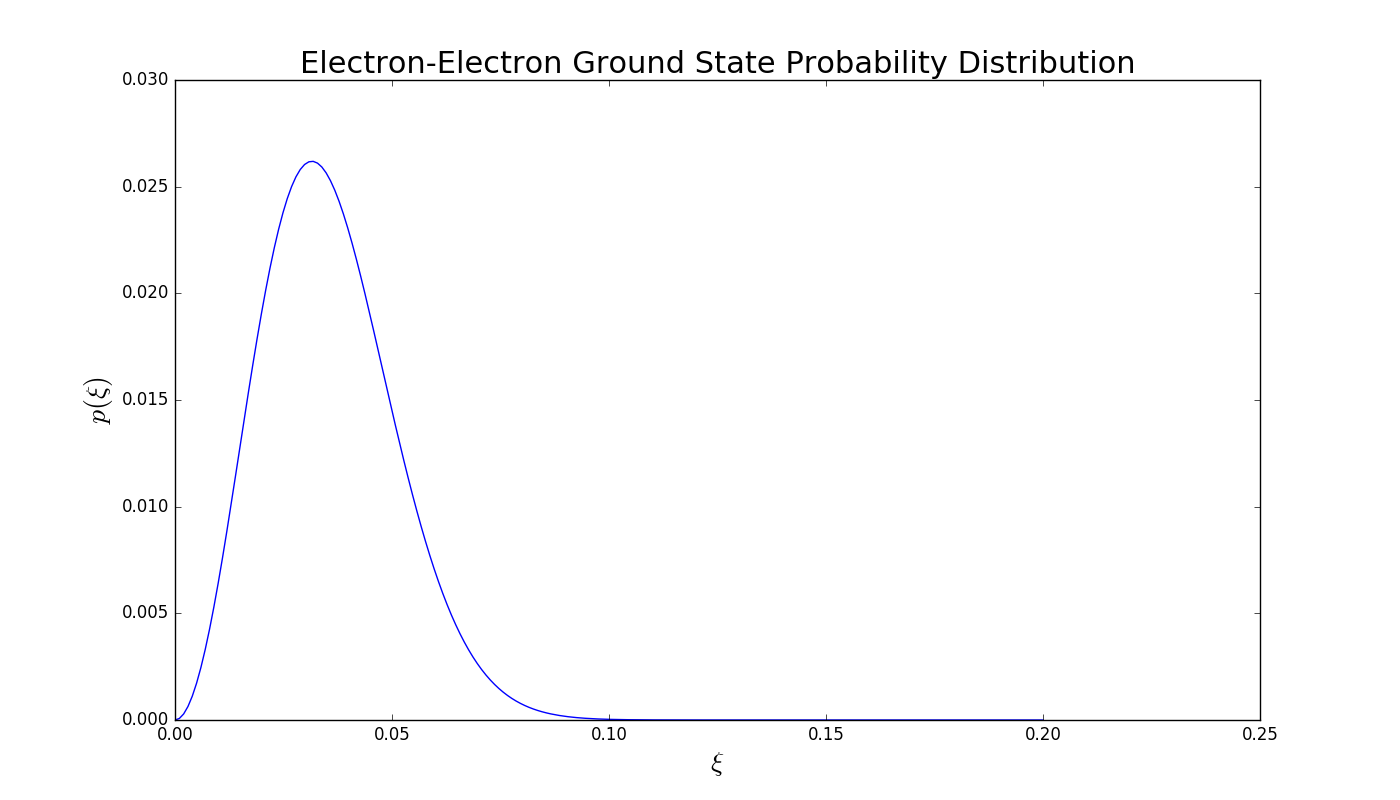
\includegraphics[scale=0.275]{InteractingElectrons/plots/prob200_10.png}
\caption{The radial ground state of the Coulomb-interacting electron-electron quantum harmonic oscillator. Here, infinity is approximated by \(\xi_\infty=0.2\) and the harmonic oscillator frequency is \(\omega=1.0\).}
\label{fig:interactingelectrons_eigenvectors2}
\end{figure}
\begin{figure}[h!]
\centering
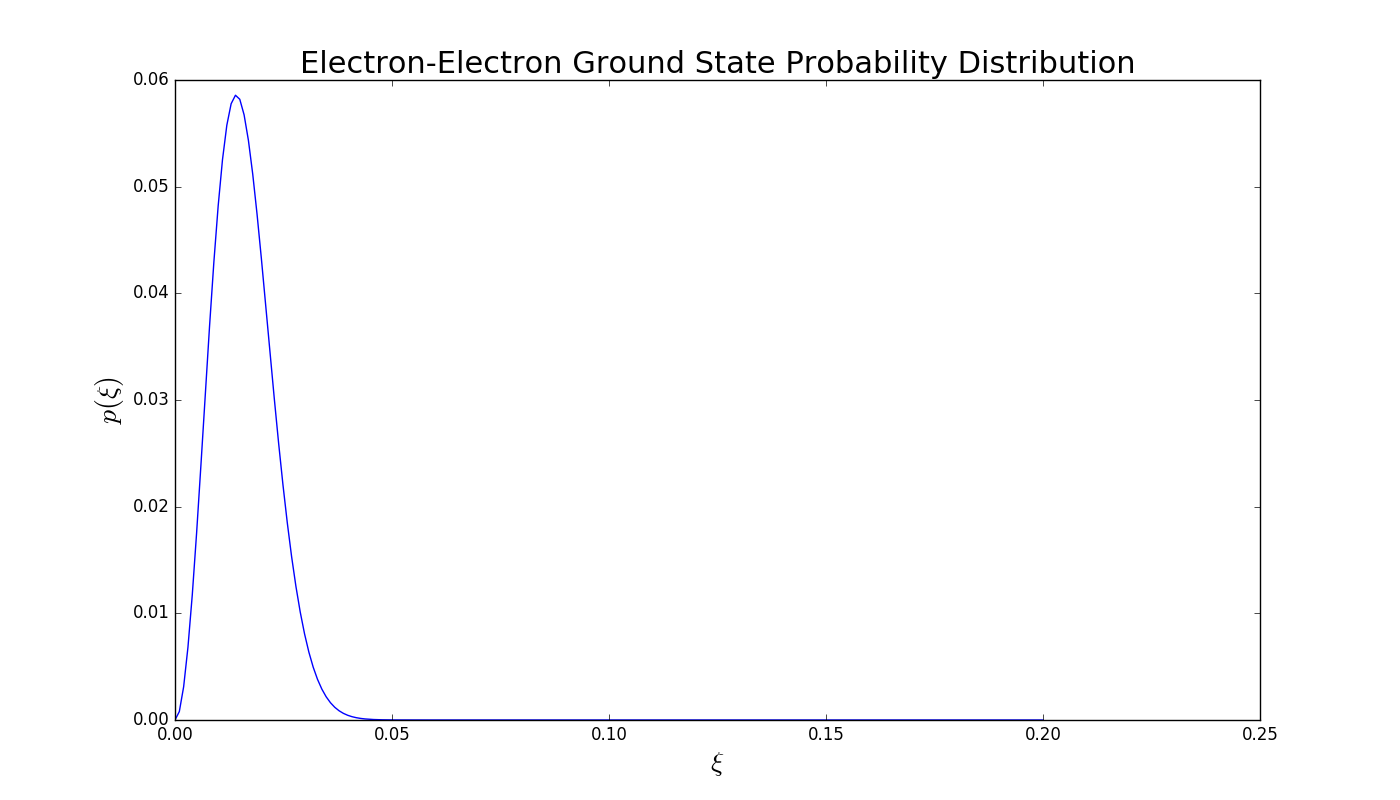
\includegraphics[scale=0.275]{InteractingElectrons/plots/prob200_50.png}
\caption{The radial ground state of the Coulomb-interacting electron-electron quantum harmonic oscillator. Here, infinity is approximated by \(\xi_\infty=0.2\) and the harmonic oscillator frequency is \(\omega=2.5\).}
\label{fig:interactingelectrons_eigenvectors3}
\end{figure}
\section{Discussion}


\section{Conclusion}

\nocite{lecture_ode}\nocite{lecture_linalg}
\bibliographystyle{plain}
\bibliography{references}
\end{document}
